\section{Management von Betriebsdaten im Industriebetrieb}\label{sec:usecase}

\todo{Aufgaben im Industriebetrieb}
Die Aufgaben eines Industriebetriebs sind primär in der Entwicklung und Herstellung neuer verkaufsfähiger Produkte zu sehen. Zum einem werden die wertschöpfenden Aufgaben von administrativen Aufgaben des Personalwesens, der Finanzbuchhaltung sowie des Controllings und zum anderen von Serviceaufgaben im Rahmen der Instandhaltung, der Wartung und des Aftersales begleitet. Die Hauptaufgaben eines Industriebetriebs lassen sich in technisch orientierte Aufgaben innerhalb der Produktentstehung und betriebswirtschaftlich orientierte Aufgaben im Rahmen der Auftragsabwicklung differenzieren.

Der Prozess der Produktentstehung umfasst im weitesten Sinne alle Aufgaben, die ab der Produktidee bzw. der konkreten Kundenanforderung bis hin zur Qualitätssicherung anfallen, also die im Rahmen der Entwicklung/Konstruktion, der Arbeitsplanung, der NC-Program- mierung mit anschließender Fertigung und Montage und innerhalb der Qualitätssicherung (Sicherstellung der quantitativ geforderten Anforderungen) entstehenden Aufgaben.

Der Prozess der Auftragsabwicklung umfasst im weitesten Sinne alle Aufgaben von der Auftragsannahme über die (Vor-)kalkulation, über die Materialwirtschaft, die Zeit- und Kapazitätswirtschaft, die Auftragsfreigabe, die Fertigungssteuerung mit der anschließenden Fertigung und Montage und der möglichen Betriebsdatenerfassung bis hin zur Auslieferung des Produkts zum Kunden, inklusive Recnungsschreibung.

Das Qualitätswesen hat sich zunehmend von der reinen Prüfung des Produkts nach dessen Fertigstellung hin zu einer planenden und vor- ausschauenden Qualitätssicherung im gesamten Produktentstehungsprozess weiterentwickelt. Dabei müssen sowohl die technische Sicherheit des Produkts als auch die Einsatztauglichkeit beim Kunden gewährleistet sein. Ziel der Qualitätssicherung ist es, zunächst in Abstimmung mit dem Kundenwunsch Qualitätsvorgaben an das Produkt zu definieren und anschließend deren Einhaltung im Rahmen der Leistungserstellung sicherzustellen.

In Anlehnung an DIN 55350, Teil 11, können die umfassenden Aufgaben der Qualitätssicherung in die Bereiche Qualitätsplanung, -lenkung und -prüfung unterteilt werden. Unter der Qualitätsplanung sind alle Maßnahmen im Rahmen der Auswahl, Klassifizierung und Gewichtung von Qualitätsmerkmalen sowie im Rahmen der Ableitung der entsprechenden Prüfmerkmale im Hinblick auf die korrekte Messung des Erfüllungsgrads der vom Kunden bzw. Produkt gestellten Anforderungen zu verstehen. Die Qualitätslenkung hat die Aufgabe, die Einhaltung der Qualitätsvorgaben (anhand der Ergebnisse der Qualitätsprüfung) zu überwachen und nötigenfalls mit geeigneten Korrekturmaßnahmen einzugreifen.
\todo{ERP System und SAP S/4HANA erklären}
In der Produktion laufen zum einen die technisch orientierten Informationen mit den betriebswirtschaftlich orientierten Informationen eines Industriebetriebs zusammen, und zum anderen kommt es zu einer Verschmelzung von Informations- und Materialfluss innerhalb der physischen Produkterstellung.

In den der Produktion vorgelagerten Bereichen stehen vor allem die Gestaltung des Informationsflusses von Vertrieb, Einkauf, Material wirtschaft, Entwicklung, Arbeitsplanung, Produktionsplanung usw sowie die möglichst konsistente und redundanzoptimierte Nutzung von gemeinsamen Grunddaten, wie z. B. Stücklisten, Arbeitsplänen Fertigungsmitteln und Arbeitsplätzen im Vordergrund. Die Hauptaufgaben im kapitalintensiven Produktionsbereich sind hingegen die Optimierung des Maschinenparks (Fertigungs-, Montage-, Qualitätsprüfungs-, Instandhaltungsmaschinen usw.) sowie die durchgängige Gestaltung des Materialflusses. Aus informationstechnischer Sicht sind im Produktionsbereich die Steuerungsanweisungen der Produktionseinrichtungen (Werkzeugmaschinen, Industrieroboter, Transport- und Lagersysteme, flexible Fertigungszellen, Transferstraßen usw.) eng mit der zeitlichen und örtlichen Steuerung der Kunden- und Fertigungsaufträge sowie mit der Rückmeldung innerhalb der Betriebsdatenerfassung verbunden.


\todo{wichtig}


Die steigenden Ansprüche der Käufer sowie das möglichst schnelle Reagieren auf veränderte Kundenwünsche spiegeln sich in immer komplexer werdenden Produkten und Produktionsmaschinen in Industriebetrieben bzw. industriellen Unternehmen mit mechanischer Produktion wider. In zunehmendem Maße werden deshalb Programme und Maschinenanlagen für rechnergestützte und flexibel automatisierbare Produktionsabläufe eingesetzt. 




\missingfigure{Wertschöpfungskette}

In einem Industriebetrieb läuft die Aufgabenerfüllung der Auftragsabwicklung und der Produktentstehung – hoffentlich abgestimmt – zunächst parallel ab. Lediglich in der Projekteinzelfertigung sind diese Aufgaben schon zu einem frühen Zeitpunkt eng miteinander verzahnt. Spätestens im Produktionsbereich werden die Aufgaben der Auftragsabwicklung und die Aufgaben der Produktentstehung integrativ abgearbeitet. Wird z. B. ein Produkt innerhalb der Produktentstehung fertiggestellt, erfolgt mit der Rückmeldung im Rahmen der Betriebsdatenerfassung die Fortschreibung in den betriebswirtschaftlichen Daten der Auftragsabwicklung. Die zunehmende Durchdringung von Industriebetrieben im Produktionsbereich mit IT-Systemen führte zum Modell der computerintegrierten Fertigung – Computer-integrated Manufacturing (CIM).

Computer-integrated Manufacturing bezeichnet ein Konzept aus der Praxis, das sich mit der integrierten Informationsverarbeitung für betriebswirtschaftliche und technische Aufgaben in einem Industriebetrieb befasst. 

\cite{Scheer.1990} CIM

Ein charakteristisches Merkmal zur Beschreibung der Produktionsart ist die Häufigkeit der gleichen Leistungserstellung in der Produktion, also der Grad der Vervielfältigung in einer Periode sowie der Grad der Bestimmtheit der Wiederkehr derselben Leistungsart. Auf das Problem der genauen Abgrenzung zwischen Massen-, Großserien-, Mittel-, Kleinserien- und Einzelfertigung weist Schäfer (siehe Schäfer 1983) in seiner Arbeit »Der Industriebetrieb« hin.


\todo{Zitieren relevanz bauernhanze Die vier Lebenszyklen der Produktion  \cite{Bauernhansl.2014} und \cite{Wagner.2018} kapitel Erst Lean-Management, dann Industrie 
4.0! und \cite{Huber.2016}}
\subsection{Geschäftsprozesse in der Produktionsplanung und -steuerung}

Industriebetriebe mit mechanischer Fertigung befinden sich unter anderem in den Branchen Maschinen- und Anlagenbau, in der Automobilindustrie sowie in der Luftfahrtindustrie. Das Spektrum reicht hier von einfachen Einzelteilen bis hin zu komplexen Großanlagen (siehe Kagermann/Keller 2001, S. 29–48; S. 69–96; S. 127–144). Ins- besondere der deutsche Mittelstand ist eine tragende Säule im Maschinen- und Anlagenbau und durch eine tiefe Spezialisierung und Exportorientierung gekennzeichnet. So müssen hochqualifizierte Mitarbeiter den verschiedensten Anforderungen des Markts und des Gesetzgebers mit einer flexiblen Fertigungs- und Software- technologie Rechnung tragen.

SAP ERP zeichnet sich durch ein umfassendes betriebswirtschaftliches Leistungsangebot, durch hohe Modularität bei gleichzeitiger Integration der einzelnen Komponenten, durch die Unterstützung internationaler Anforderungen mittels Anbieten von entsprechender landesspezifischer Funktionalität (z. B. Personalabrechnung in verschiedenen Ländern aufgrund unterschiedlicher Gesetze und Steuersätze) und Mehrsprachigkeit sowie durch die Lauffähigkeit auf verschiedenen Rechnerplattformen aus.

SAP ERP basiert auf einer dreistufigen Client-Server-Architektur und kann in zwei Aufgabengebiete unterteilt werden: die Basisaufgaben und die betriebswirtschaftlichen Anwendungsaufgaben. Aufgabe der Basisschicht ist es, die betriebswirtschaftlichen Anwendungen unabhängig von den Systemschnittstellen des Betriebs- sowie des Datenbank- und Kommunikationssystems zu gestalten und für eine performante Abwicklung der betriebswirtschaftlichen Transaktionen zu sorgen. In der Anwendungsschicht ist das implementierte Lösungsangebot zur Unterstützung der betriebswirtschaftlichen Anforderungen der Unternehmen enthalten.

Die Fertigungsart bzw. Produktionsart charakterisiert die Häufigkeit der Leistungswiederholung im Produktionsprozess. Charakterisie- rende Merkmale zur Bestimmung der Fertigungsart sind die Wiederholhäufigkeit gleicher oder ähnlicher Produkte sowie die Auflagen- höhe der Fertigungsaufträge. Eng verbunden mit der Fertigungsart ist die Fertigungsorganisation, da nicht selten die Fertigungsart maßgeb- lichen Einfluss auf die Gestaltung des Fertigungsablaufs hat. 

Im Wesentlichen umfassen die Prozesse in der Produktionsplanung 
und -steuerung die folgenden Bereiche:

\begin{itemize}
    \item 
    Absatz- und Produktionsgrobplanung zur Festlegung der zu produzierenden Mengen
    \item 
    Materialbedarfsplanung zur Nettobedarfsrechnung und Ermittlung der Komponentenbedarfe unter Berücksichtigung von Ausschuss und Losgrößen
    \item 
    Kapazitätsplanung zur Feinplanung der Produktion unter Berücksichtigung der verfügbaren Kapazitäten
    \item 
    Fertigungssteuerung zur Steuerung und Erfassung der Fertigungsdurchführung (Erstellung der Fertigungspapiere, Erfassung der Rückmeldungen)
\end{itemize}


Diese vier Bereiche stellen den Prozessumfang nur sehr grob dar – einen detaillierteren Überblick gibt Abbildung \ref{fig:Prozessüberblick der Produktionsplanung und -steuerung}. Hier sind die Prozessbausteine, die wir in den folgenden Kapiteln ausführlich behandeln, explizit mit ihren wichtigsten Eingangs- und Ausgangsgrößen dargestellt.


\begin{figure}[H]
	\centering 
    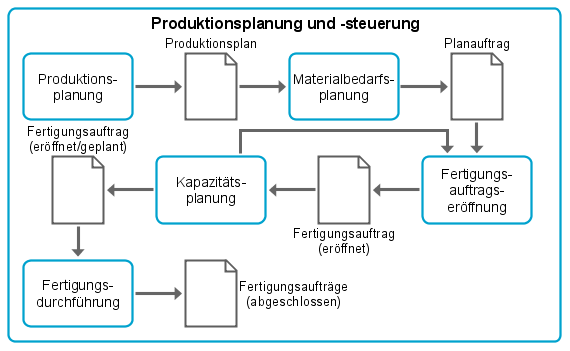
\includegraphics[width=\textwidth]{img/Produktion.png}	
    \caption[Prozessüberblick der Produktionsplanung und -steuerung]
    {Prozessüberblick der Produktionsplanung und -steuerung \protect\footnotemark}
    \label{fig:Prozessüberblick der Produktionsplanung und -steuerung}
\end{figure}
\footnotetext{in Anlehnung an \citeauthor{Dickersbach.2014} \citeyear{Dickersbach.2014} \cite{Dickersbach.2014} }


Wichtige Fertigungsarten sind (siehe Keller/Curran 1999, S. 137–154): 

diskrete Fertigung 

Serienfertigung 

Prozessfertigung 

Kanban 

Projektfertigung

\todo{nur auf diskrete eingehen, auf literatur verweisen}


\subsection{Vorstellung der Fertigungsdurchführung in der diskreten Fertigung}

\todo{Definition Fertigungsdurchführung}

\todo{Diskrete Fertigung}
Die diskrete Fertigung \todo{fußnote(auch Werkstattfertigung) } beschreibt die Fertigung eines Erzeugnisses auf der Basis von Fertigungsaufträgen. Die diskrete Fertigung kommt zum Einsatz, wenn die zu produzierenden Erzeugnisse häufig wechseln, wenn die Bedarfe sehr unregelmäßig auftreten und die Fertigung einen werkstattorientierten Ablauf hat. Um eine diskrete Fertigung durchführen zu können, sind eine Reihe von Stammdaten erforderlich. Zu den wichtigsten Stammdaten gehören Material, Stückliste, Arbeitsplatz und Arbeitsplan.

Die diskrete Fertigung beginnt mit der Eröffnung und Bearbeitung eines Fertigungsauftrags. Die Eröffnung des Fertigungsauftrags kann entweder durch Umsetzen eines in der Produktions- und Beschaffungsplanung erzeugten Planauftrags oder durch dessen manuelles Anlegen erfolgen. Ein Fertigungsauftrag ist eine Anforderung an die Produktion, Materialien bzw. Leistungen zu einem bestimmten Termin in einer bestimmten Menge herzustellen bzw. zu erbringen. Er legt fest, auf welchem Arbeitsplatz und mit welchen Einsatzmaterialien das entsprechende Material zu fertigen ist. Das Eröffnen eines Fertigungsauftrags erzeugt automatisch Materialreservierungen für die benötigten Materialkomponenten. Für fremdzubeschaffende Materialkomponenten bzw. Dienstleistungen werden Bestellanforderungen erstellt. An den Arbeitsplätzen, an denen der Auftrag durch- geführt wird, entstehen Kapazitätsbelastungen.

Die Fertigungsaufträge werden bei Erreichen des Freigabetermins und bei vorhandener Material- und Kapazitätsverfügbarkeit freigegeben. Zur Vorbereitung der Durchführung können die entsprechenden Papiere des Fertigungsauftrags ausgedruckt werden. Die Auswertung der Kapazitätssituation und der gegebenenfalls notwendige Kapazitätsabgleich können in jeder Phase der Fertigungsauftragsabwicklung durchgeführt werden. Meist geschieht dies, bevor mit der Fertigung begonnen wird. Die zur Produktion der Erzeugnisse benötigten Komponenten werden aus dem Fertigungsauftrag entnommen, und der Warenausgang wird gebucht. Nun wird das Erzeugnis anhand des Fertigungsauftrags produziert. Die gefertigte Menge und die erbrachten Leistungen werden dem Fertigungsauftrag zurückgemeldet, das Erzeugnis auf Lager gelegt und der Wareneingang gebucht. Zum Abschluss wird der Fertigungsauftrag abgerechnet.

\missingfigure{Prozessüberblick}
Die Fertigungsauftragseröffnung leitet die kurzfristigen Aufgaben der Fertigungssteuerung ein. 
Die Fertigungsdurchführung wird mit der Auftragsfreigabe eingeläutet. Diese bewirkt eine Statusänderung des Fertigungsauftrags und ist die systemtechnische Voraussetzung für die nachfolgenden Schritte – vom Auftragsdruck über die Materialentnahme für die Komponenten, über die Rückmeldung bis hin zum Lagerzugang sowie über die Abrechnung bis hin zum Abschluss. Bei der Freigabe kann erneut eine Verfügbarkeitsprüfung erfolgen.

Die Aufgabe des Fertigungsauftrags ist es, sowohl die Fertigung zu steuern als auch die Fertigung mengen- und kostenmäßig zu erfassen. Zur Steuerung der Fertigung gehört unter anderem die Bereitstellung der Information, welches Produkt in welcher Menge mit welchen Ressourcen zu welchem Zeitpunkt gefertigt werden soll. Hierzu ist es erforderlich, dass der Fertigungsauftrag Stammdaten und Steuerungsparameter enthält. Entsprechend den Stammdaten Arbeitsplan und Stückliste gliedert sich der Fertigungsauftrag im Wesentlichen in:

Kopfdaten, die organisatorische Informationen, wie die Auftragsnummer, sowie Kosten, Mengen und Termine für den Auftrag als Ganzes enthalten 

Vorgangsdaten, die detaillierte Vorgangstermine, Vorgabewerte und auch die rückgemeldeten Mengen und Termine enthalten 

Komponentendaten zu den Vorgängen wie Bedarfsmenge und Reservierungsnummer

Im Produktionsbereich treffen sich innerhalb der Fertigungsdurch- führung die bisher teilweise unterschiedlich verlaufenen Informa- tions- und Materialflüsse. Sind sämtliche für die Produktion benötig- ten Unterlagen (wie z. B. Zeichnung, Stückliste, Arbeitsplan mit seinen Kalkulationswerten, Fertigungsauftrag und Personalressour- cen) vorhanden und steht der Fertigungstermin unmittelbar bevor, müssen Sie dafür Sorge tragen, dass die fremd- und eigenbeschafften Rohmaterialien und Einbauteile physisch vorhanden, für die Produk- tion freigegeben und zur Produktionsstätte geliefert worden sind. Sind die Materialien, die Fertigungs- und Fertigungshilfsmittel sowie das Personal vor Ort, kann mit der physischen Produkterstellung begonnen werden.

\todo{rollen}
Während die in Abschnitt 3.3 aufgeführten Planer ausschließlich für die Stammdatenpflege zuständig sind, liegt die Produktionsplanung und -steuerung im Aufgabenbereich der Planer Disponent, Kapazitätsplaner und Fertigungssteuerer. Diese drei Planer entsprechen den Rollen, die SAP für die Produktionsplanung und -steuerung vorsieht – in einem Unternehmen können einer Person mehrere oder sogar alle Rollen zugeordnet sein. Die Bedeutung dieser Rollen liegt in erster Linie darin, dass sie eine schnelle Auswahl von Planungsobjekten nach Zuständigkeit erlaubt.

Im Produktionsbereich treffen sich innerhalb der Fertigungsdurchführung die bisher teilweise unterschiedlich verlaufenen Informations- und Materialflüsse. Sind sämtliche für die Produktion benötigten Unterlagen (wie z. B. Zeichnung, Stückliste, Arbeitsplan mit seinen Kalkulationswerten, Fertigungsauftrag und Personalressourcen) vorhanden und steht der Fertigungstermin unmittelbar bevor, müssen Sie dafür Sorge tragen, dass die fremd- und eigenbeschafften Rohmaterialien und Einbauteile physisch vorhanden, für die Produktion freigegeben und zur Produktionsstätte geliefert worden sind. Sind die Materialien, die Fertigungs- und Fertigungshilfsmittel sowie das Personal vor Ort, kann mit der physischen Produktherstellung begonnen werden.


Die Fertigungsdurchführung schließt an die Fertigungsauftragseröffnung oder an die Kapazitätsplanung an. Basierend auf Fertigungsauf- trägen mit festen Vorgangsterminen wird mit der Freigabe des Fertigungsauftrags der systemseitige Startschuss zur Durchführung der Fertigung gegeben. Zusammen mit der Freigabe wird in der Regel eine Verfügbarkeitsprüfung durchgeführt. Der Auftragsdruck erfolgt entweder ebenfalls mit der Freigabe oder im Anschluss daran in einem separaten Schritt. Die nachfolgenden Schritte sind die Materialentnahme der Komponenten, die Rückmeldung der erfolgten Fertigungsschritte – inklusive der Gutmengen und des Ausschusses – sowie der Lagerzugang. Die Fertigungsaufträge bleiben im System, bis sie archiviert oder gelöscht worden sind. An abgeschlossenen Fertigungsaufträgen ist keine Änderung mehr möglich.

\todo{Alternative MES}
Eine abweichende, jedoch ebenfalls gebräuchliche Vorgehensweise ist es, die erstellten und freigegebenen Fertigungsaufträge an ein Prozessleitsystem weiterzugeben, dort die eigentliche Fertigungssteuerung inklusive der kapazitiven Planung vorzunehmen und die Rückmeldung der Fertigungsaufträge an PP weiterzugeben. In diesem Fall wird die Produktionsplanungs- und -steuerungsfunktionalität von SAP ERP hauptsächlich für die Materialbedarfsplanung, für die Bestandsrechnung und für die Kostenabrechnung verwendet.

Zur Verringerung des Pflegeaufwands kann der Wareneingang mithilfe der Rückmeldung des letzten Auftrags automatisch gebucht werden. Hierzu ist keine Endrückmeldung erforderlich; Der automatische Wareneingang funktioniert auch für teilrückgemeldete Mengen.

Im Rahmen dieser Bachelorarbeit soll die \todo{Für die was?} für einen ausgewählten Teil des Geschäftsprozesses \textit{Fertigungsdurchführung} erfolgen.


Im Rahmen der Betriebsdatenerfassung (BDE) werden die realisierten Mengen- und Zeitwerte der Aufträge und Mitarbeiter, Stillstands- und Ausfallzeiten von Betriebsmitteln sowie der Einsatz von Materialien und Werkzeugen in den Planungs- und Steuerungsprozeß zurückgemeldet. Insbesondere eine zeitnahe Werkstattsteuerung setzt auch die laufende Information über den Ist-Zustand des Produktionsprozesses voraus. Für die Betriebsdatenerfassung werden spezielle Hardwaresysteme wie störungsunanfällige Terminals oder automatische Signalgeber an Produktionsanlagen eingesetzt, die zum Teil auch einen Prozeßrechner erfordern. Aus diesem Grunde führen BDE-Systeme in der Regel zu einer Vernetzung von mehreren Rechnersystemen.

